\documentclass[conference]{IEEEtran}
\IEEEoverridecommandlockouts
\renewcommand{\thesection}{\Roman{section}}
\usepackage{cite}
\usepackage{amsmath,amssymb,amsfonts}
\usepackage{booktabs}
\usepackage{array}
\usepackage{graphicx}
\usepackage{textcomp}
\usepackage{xcolor}
\usepackage{tikz}
\usetikzlibrary{positioning,arrows.meta,calc,fit,backgrounds}
\usepackage{pgfplots}
\pgfplotsset{compat=1.17}
\usepackage[ruled,vlined]{algorithm2e}
\usepackage[hidelinks]{hyperref}

\pagestyle{empty}

\title{An Empirical Analysis of Entangled Enhancement in an Autonomous Driving Pipeline of ML Components}

\author{\IEEEauthorblockN{Rashedul Arefin Ifty, Fumio Machida}
\IEEEauthorblockA{University of Tsukuba\\
Tsukuba, Japan\\
ifty.rashedul@sd.cs.tsukuba.ac.jp, machida@cs.tsukuba.ac.jp}}

\begin{document}
\maketitle
\thispagestyle{empty}
\bstctlcite{IEEEexample:BSTcontrol}% disable the dash for repeated author names

% ============================================================================
% STEP 1 SKELETON: every paragraph below is a planned topic sentence.
% Each topic sentence becomes one paragraph in Steps 2 to 6.
% ============================================================================

\begin{abstract}
Entangled enhancement is a retraining that improves one component of a machine
learning system (MLS) but fails to improve the whole system. This paper
measures entangled enhancement in an autonomous driving pipeline in which the
perception, prediction and planning modules are all ML components. The
perception module is updated 30 times on data from a new city, and every update improves the perception module. The prediction and planning modules
are trained once, either on the ground truth or on the output of the old perception module, and stay fixed. When the prediction
module was trained on the output of the old perception module, the prediction
error increased in 23 of the 30 updates, in 11 above random variation and in 3
with a bootstrap interval above zero. When the prediction module was trained on
the ground truth, the counts were 5, 0 and 0. The planning error changed by at
most 0.13\,m. No label-free measure of output change predicted which updates harmed the prediction module.
\end{abstract}

\begin{IEEEkeywords}
autonomous driving, entangled enhancement, machine learning system, model maintenance, retraining
\end{IEEEkeywords}

% ============================================================================
\section{Introduction}
% ============================================================================

An MLS is often built as a pipeline, which is a set of ML components connected
in a line, where each component uses the output of the preceding component. A
component that comes earlier in the line is upstream of a component that comes
later, and the later component is downstream. Retraining an upstream component
can improve that component and still fail to improve the whole system. Wang and
Machida call this effect entangled enhancement and model when an MLS should
retrain each component~\cite{wang2024compsac,wang2025issre}. The models of Wang and Machida need the probability that retraining the upstream component leaves the downstream
component working, and this probability has not been measured on a real
system.

A driving pipeline has three components. The perception module finds the
objects around the ego vehicle, which is the vehicle that the pipeline drives.
The prediction module predicts where each object will move, and the planning
module chooses the path of the ego vehicle. The three modules are trained
separately and are updated one at a time. An earlier experiment in this study
retrained the perception module of such a pipeline 15 times, and the planning
error increased in 6 of the 15 updates. The prediction module and the planning
module in that pipeline were fixed rules. Fixed rules cannot adapt to the
mistakes of the perception module, and that experiment could not test the
adaptation that the theory of entangled enhancement describes.

This paper replaces both fixed rules with ML components. The ground truth is
the set of object positions labelled by hand. The prediction module and the
planning module are trained in two ways, once on the ground truth and once on
the output of the old perception module. Only the second way allows the
downstream modules to adapt to the old mistakes. The comparison of the two ways
therefore shows whether a harm after an update comes from that adaptation.

This paper makes three contributions.
\begin{enumerate}
\item A driving pipeline of three ML components, trained on a reduced
nuScenes dataset and checked against simple baselines.
\item A campaign of 30 updates of the perception module, with the number of
harmful updates counted at three levels of evidence.
\item A test of nine measures of output change that need no ground truth, as a
possible symptom of entangled enhancement.
\end{enumerate}

% ============================================================================
\section{Background and Related Work}
% ============================================================================

This section summarises the earlier work that the experiment builds on.
Sculley et al.~\cite{sculley2015hidden} describe how a change to one component
of an MLS changes the behaviour of every component that uses the changed
output. Wu et al.~\cite{wu2021fixesthatfail} show that improving one model of a
system can make the whole system worse. A harm of this kind can have two
causes. In the first cause, the downstream components adapted during training
to the mistakes of the old upstream component and are disturbed when those
mistakes change. In the second cause, the upstream component improves on
average but becomes worse on the cases that matter downstream.

AutoBots~\cite{girgis2022autobots} predict the future of one target object from
the past positions of the surrounding objects, and PlanT~\cite{renz2022plant}
plans the path of the ego vehicle from a list of object tokens. Weng et
al.~\cite{weng2022whose} show that a prediction module can learn by attention
which detections belong to the same object. The prediction error increases
when the input comes from a real perception module instead of the ground
truth~\cite{xu2024realworld}. A planning module that receives
the state of the ego vehicle can score well on nuScenes while ignoring the
objects~\cite{zhai2023rethinking,li2024egostatus}.

Rabanser et al.~\cite{rabanser2019failing} detect a change in the data seen by
a model without ground truth from distances between distributions, where a
distribution is the pattern of values that an output takes over many inputs.
This paper applies such distances to the outputs of the perception module and
of the prediction module as a candidate symptom of entangled enhancement.

% ============================================================================
\section{Methodology}
% ============================================================================

This section defines the notation, states the two hypotheses, and describes
the workflow and the procedure that test the hypotheses.

\subsection{Pipeline and Notation}
The perception module $C_1$ finds the objects in the image of the front camera.
The prediction module $C_2$ predicts the path of each object over the next
3\,s, and the planning module $C_3$ chooses the path of the ego vehicle over
the same 3\,s. An update is one retraining of $C_1$ on data from a new city. We
call $C_1$ before an update the old $C_1$ and $C_1$ after the update the new $C_1$.

We write $\delta_1$ for the gain of $C_1$ in mAP50, the standard accuracy
measure for object detection. The prediction error is the minADE, which is the
average distance between the predicted path and the true path of an object,
taken for the best of the paths that $C_2$ predicts. The planning error is the
distance between the planned position and the position of the human driver at
3\,s. We write $\Delta_2$ and $\Delta_3$ for the increase of the prediction
error and of the planning error after an update. An update shows entangled
enhancement when
\begin{equation}
\delta_1 > 0 \quad \text{and} \quad (\Delta_2 > 0 \ \text{or} \ \Delta_3 > 0).
\label{eq:ee}
\end{equation}

\subsection{Hypotheses}
\noindent\textbf{H1 (existence):} An update of $C_1$ can increase the
prediction error or the planning error of a pipeline of three ML components,
even when the update makes $C_1$ more accurate. The increase is larger when
$C_2$ and $C_3$ were trained on the output of the old $C_1$ than when $C_2$ and
$C_3$ were trained on the ground truth.

\noindent\textbf{H2 (symptom):} The change in the output of $C_1$ and $C_2$
after an update, measured without ground truth, is larger for the updates that
meet condition~(\ref{eq:ee}) than for the other updates. The gain $\delta_1$
alone does not separate the two groups. If H2 holds, an engineer can compute
the change before using an update and retrain $C_2$ and $C_3$ when the change
is large.

\subsection{Workflow}
Fig.~\ref{fig:workflow} shows the six stages of the experiment. The old $C_1$
is trained with two random seeds, where a random seed is the starting number
for the random choices made during training. $C_2$ and $C_3$ are trained once
along two routes. Route A uses the ground truth, and route B uses the output
of the old $C_1$. Each of the 30 updates is then tested in the full pipeline
with $C_2$ and $C_3$ kept fixed.

\begin{figure*}[t]
\centering
\resizebox{\textwidth}{!}{%
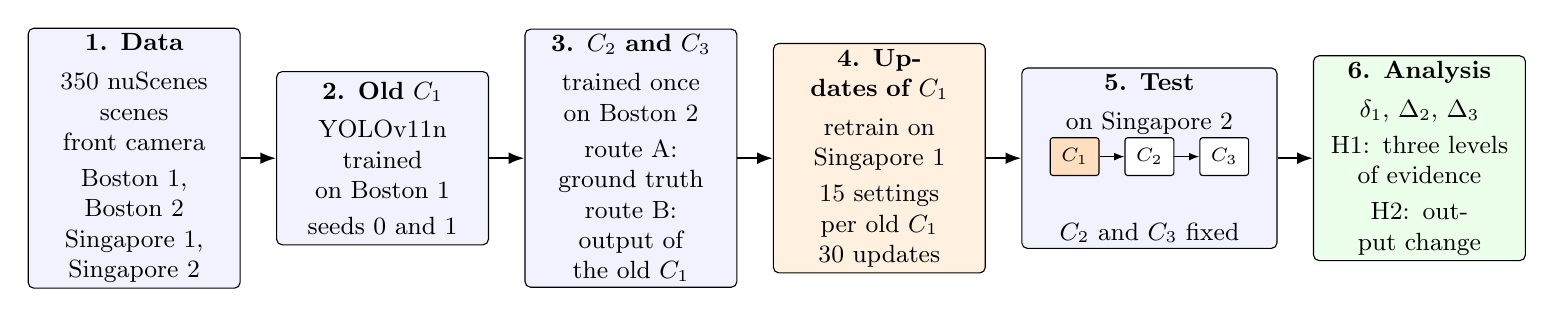
\begin{tikzpicture}[
  font=\small,
  stage/.style={draw, rounded corners=2pt, fill=blue!5, align=center,
                text width=2.55cm, minimum height=2.2cm, inner sep=2pt},
  head/.style={font=\small\bfseries, align=center},
  arr/.style={-{Latex[length=2mm]}, thick},
  mod/.style={draw, rounded corners=1pt, fill=white, minimum width=0.62cm,
              minimum height=0.48cm, inner sep=1pt, font=\scriptsize},
]
\node[stage] (s1) at (0,0) {\textbf{1. Data}\\[3pt] 350 nuScenes scenes\\ front camera\\[2pt] Boston 1, Boston 2\\ Singapore 1, Singapore 2};
\node[stage, right=0.45cm of s1] (s2) {\textbf{2. Old $C_1$}\\[3pt] YOLOv11n trained\\ on Boston 1\\[2pt] seeds 0 and 1};
\node[stage, right=0.45cm of s2] (s3) {\textbf{3. $C_2$ and $C_3$}\\[3pt] trained once on Boston 2\\[2pt] route A: ground truth\\ route B: output of\\ the old $C_1$};
\node[stage, right=0.45cm of s3, fill=orange!12] (s4) {\textbf{4. Updates of $C_1$}\\[3pt] retrain on Singapore 1\\[2pt] 15 settings per old $C_1$\\ 30 updates};
\node[stage, right=0.45cm of s4, text width=3.1cm] (s5) {\textbf{5. Test}\\[3pt] on Singapore 2\\[16pt] \phantom{x}\\[2pt] $C_2$ and $C_3$ fixed};
\node[stage, right=0.45cm of s5, fill=green!8] (s6) {\textbf{6. Analysis}\\[3pt] $\delta_1$, $\Delta_2$, $\Delta_3$\\[2pt] H1: three levels\\ of evidence\\[2pt] H2: output change};
\foreach \a/\b in {s1/s2,s2/s3,s3/s4,s4/s5,s5/s6} \draw[arr] (\a) -- (\b);
% small pipeline inside stage 5
\node[mod, fill=orange!25] (p1) at ($(s5.center)+(-0.95,0.02)$) {$C_1$};
\node[mod] (p2) at ($(s5.center)+(0,0.02)$) {$C_2$};
\node[mod] (p3) at ($(s5.center)+(0.95,0.02)$) {$C_3$};
\draw[-{Latex[length=1.3mm]}] (p1) -- (p2);
\draw[-{Latex[length=1.3mm]}] (p2) -- (p3);
\end{tikzpicture}}
\caption{Workflow of the experiment}
\label{fig:workflow}
\end{figure*}

\subsection{Campaign Procedure}
Algorithm~\ref{alg:campaign} gives the procedure for one old $C_1$. The random
variation $\tau_2$ and $\tau_3$ is the largest change of the errors when the
old $C_1$ is replaced by the other old $C_1$, which differs only in the random
seed. The first level of evidence counts any increase, and the second level
counts an increase above the random variation. The third level counts an
increase whose 95\,\% bootstrap interval lies above zero. The bootstrap
repeats the measurement on test sets drawn with replacement from the test
scenes.

\begin{algorithm}[t]
\footnotesize
\DontPrintSemicolon
\SetKwInOut{Input}{Input}\SetKwInOut{Output}{Output}
\Input{old $C_1^{\mathrm{old}}$, settings $\mathcal{S}$, Boston~2, Singapore~1, Singapore~2}
\Output{$\delta_1$, $\Delta_2$, $\Delta_3$ and evidence level per update and route}
Train $C_2^{A}, C_3^{A}$ on the ground truth of Boston~2\;
Train $C_2^{B}, C_3^{B}$ on the output of $C_1^{\mathrm{old}}$ on Boston~2\;
\ForEach{route $r \in \{A, B\}$}{
  $E_2^{r}, E_3^{r} \leftarrow$ errors of $C_1^{\mathrm{old}} \rightarrow C_2^{r} \rightarrow C_3^{r}$ on Singapore~2\;
}
$\tau_2, \tau_3 \leftarrow$ random variation from the other old $C_1$\;
\ForEach{setting $s \in \mathcal{S}$}{
  $C_1^{\mathrm{new}} \leftarrow$ retrain $C_1^{\mathrm{old}}$ on Singapore~1 with $s$\;
  $\delta_1 \leftarrow \mathrm{mAP50}(C_1^{\mathrm{new}}) - \mathrm{mAP50}(C_1^{\mathrm{old}})$\;
  \ForEach{route $r \in \{A, B\}$}{
    $\Delta_2, \Delta_3 \leftarrow$ errors of $C_1^{\mathrm{new}} \rightarrow C_2^{r} \rightarrow C_3^{r}$ minus $E_2^{r}, E_3^{r}$\;
    record the three levels of evidence\;
  }
  record the output change of $C_1$ and $C_2$ for H2\;
}
\caption{Update campaign for one old $C_1$}
\label{alg:campaign}
\end{algorithm}

% ============================================================================
\section{Experimental Setup}
% ============================================================================

This section gives the data, the updates, the ML models and the
measurements. All models were trained on one Tesla T4 graphics card.

\subsection{Data}
The experiment uses 350 of the 850 scenes of nuScenes~\cite{caesar2020nuscenes},
which are driving clips of about 20\,s from Boston and Singapore, with the
full-size images of the front camera only (4.6\,GB). Boston~1 (100 scenes) trains $C_1$, and Boston~2 (100 scenes)
trains $C_2$ and $C_3$, with 14 of the scenes kept for validation. A perception
module is much more accurate on the scenes used to train that module, and
separate scenes give $C_2$ and $C_3$ the realistic mistakes of
$C_1$~\cite{xu2024realworld}. Singapore~1 (100 scenes) is used for the updates,
and Singapore~2 (50 scenes, 2{,}020 images) is used for testing. The test set
has 1{,}720 test samples, one for every keyframe with 3\,s of future.

\subsection{Updates of the Perception Module}
$C_1$ is YOLOv11n~\cite{jocher2024yolo11}, trained for 10 passes over
Boston~1 with the random seeds 0 and 1. The two old $C_1$ reach an mAP50 of
0.109 and 0.117 on Singapore~2. An update retrains an old $C_1$ on Singapore~1
with one of 15 settings. Nine settings use 100\,\%, 50\,\% or 25\,\% of the
images (3{,}575, 1{,}788 or 894) with the seeds 1, 2 and 3 and 10 passes. Six
settings use all images with 5 or 20 passes and the same seeds. The 15 settings
applied to both old $C_1$ give 30 updates. Every update keeps the final model,
and the test scenes are never used to choose a model.

\subsection{ML Prediction and Planning Modules}
$C_2$ follows AutoBot-Ego~\cite{girgis2022autobots}. For each current object,
a transformer reads the objects of the last four keyframes relative to that
object and outputs six possible paths of 3\,s, without a hand-written
tracker~\cite{weng2022whose}. $C_3$ follows PlanT~\cite{renz2022plant}. Every
object becomes one token with the current position, the most likely path from
$C_2$, the class and the confidence. Two further tokens hold the driving
command and the path of the ego vehicle over the last 1.5\,s. The command is
left, straight or right, from the lateral position of the human path at
3\,s~\cite{zhai2023rethinking}. A four-layer encoder and a recurrent decoder
output six points of the planned path.

Both models were trained on Boston~2 with early stopping on the validation
scenes and with mirror and rotation augmentation. An input of the ego path can
let a planning module ignore the objects~\cite{li2024egostatus}, and the
experiment checks whether $C_3$ uses the objects. Removing the objects from the input of $C_3$ moves the planned
position at 3\,s by 0.73 to 1.65\,m on average, which is above the threshold of
0.5\,m fixed before the experiment.

\subsection{Training Routes and Measurements}
\label{sec:measures}
$C_2$ and $C_3$ are trained once along route A and once along route B for each
old $C_1$, and the trained models stay fixed during all updates. The prediction
error is computed over the detections that are matched one to one with a ground
truth object of the same class. The collision rate is the fraction of test
samples in which the planned path overlaps an object. The outputs of $C_2$ and
$C_3$ on the ground truth stayed exactly the same before and after every
update, which confirms that only the output of $C_1$ changed. The random
variation is $\tau_2 = 0.112$\,m and $\tau_3 = 0.018$\,m. The bootstrap draws
the 50 test scenes 2{,}000 times with replacement.

% ============================================================================
\section{Results}
% ============================================================================

This section reports the validity of the ML components, the effect of the
updates, and the test of the symptom. Every update made $C_1$ more accurate,
with $\delta_1$ between 0.048 and 0.118.

\subsection{Validity of the ML Components}
Table~\ref{tab:validity} compares $C_2$ and $C_3$ with simple baselines on the
test set. $C_2$ beats a baseline in which every object stays where the object
is, and on the ground truth $C_2$ also beats a constant-velocity extrapolation
of 1.01\,m. The variant of $C_3$ without any ego input does not beat the
baseline that drives the average Boston path for each command. The experiment
therefore uses the variant with the ego path, which has a collision rate of
0.05 to 0.08 against 0.18 for the baseline.

\begin{table}[t]
\centering
\caption{ML components against simple baselines on the test set (m)}
\label{tab:validity}
\small
\setlength{\tabcolsep}{4pt}
\begin{tabular}{@{}lcc@{}}
\toprule
\textbf{Model and input} & \textbf{Model} & \textbf{Baseline} \\
\midrule
$C_2$ on the ground truth & 0.77 & 4.48 (stays still) \\
$C_2$ on the output of $C_1$ & 2.39 to 2.95 & 5.39 to 5.85 (stays still) \\
$C_3$ without ego input & 9.3 to 12.5 & 9.25 (average path) \\
$C_3$ with the ego path & 3.70 to 4.16 & 9.25 (average path) \\
\bottomrule
\end{tabular}
\end{table}

\subsection{Prediction Module}
Fig.~\ref{fig:delta2} shows $\Delta_2$ for every update and both routes. In all
30 updates, $\Delta_2$ of route B is larger than $\Delta_2$ of route A. The
difference is largest for the updates from the old $C_1$ with seed 0, where
$\Delta_2$ of route B lies between $+0.049$ and $+0.284$\,m with a mean of $+0.165$\,m.

\begin{figure}[t]
\centering
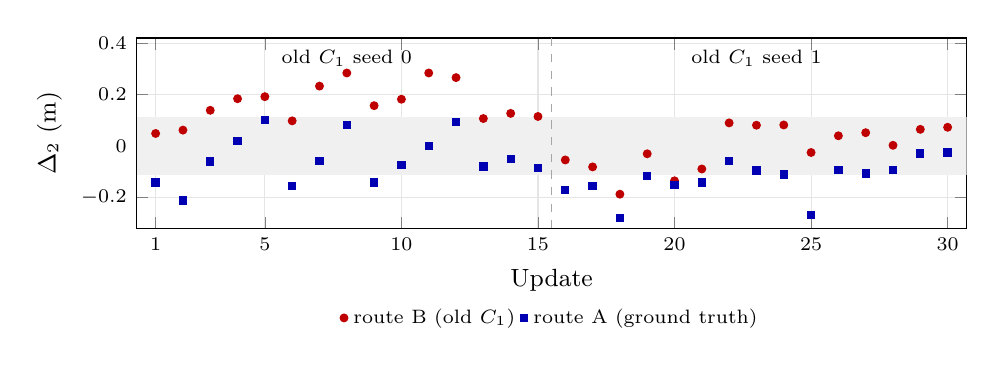
\begin{tikzpicture}
\begin{axis}[width=\columnwidth, height=4.0cm,
    xlabel={Update}, ylabel={$\Delta_2$ (m)},
    xmin=0.3, xmax=30.7, ymin=-0.32, ymax=0.42,
    xtick={1,5,10,15,20,25,30}, tick label style={font=\scriptsize},
    label style={font=\small},
    legend style={at={(0.5,-0.36)}, anchor=north, legend columns=2,
                  font=\scriptsize, draw=none},
    grid=major, grid style={gray!20}]
\fill[gray!12] (axis cs:0.3,-0.112) rectangle (axis cs:30.7,0.112);
\draw[gray!70, dashed] (axis cs:15.5,-0.32) -- (axis cs:15.5,0.42);
\addplot[only marks, mark=*, mark size=1.4pt, color=red!75!black] coordinates {
(1,0.049) (2,0.062) (3,0.139) (4,0.184) (5,0.192) (6,0.098) (7,0.233) (8,0.284) (9,0.157) (10,0.182) (11,0.284) (12,0.266) (13,0.107) (14,0.127) (15,0.115) (16,-0.054) (17,-0.081) (18,-0.187) (19,-0.030) (20,-0.135) (21,-0.089) (22,0.090) (23,0.081) (24,0.082) (25,-0.025) (26,0.040) (27,0.052) (28,0.003) (29,0.065) (30,0.073)};
\addlegendentry{route B (old $C_1$)}
\addplot[only marks, mark=square*, mark size=1.3pt, color=blue!70!black] coordinates {
(1,-0.141) (2,-0.212) (3,-0.060) (4,0.021) (5,0.100) (6,-0.154) (7,-0.058) (8,0.082) (9,-0.141) (10,-0.073) (11,0.001) (12,0.093) (13,-0.079) (14,-0.051) (15,-0.085) (16,-0.170) (17,-0.156) (18,-0.280) (19,-0.115) (20,-0.152) (21,-0.141) (22,-0.059) (23,-0.095) (24,-0.111) (25,-0.267) (26,-0.094) (27,-0.107) (28,-0.094) (29,-0.029) (30,-0.025)};
\addlegendentry{route A (ground truth)}
\node[font=\scriptsize, anchor=north] at (axis cs:8,0.41) {old $C_1$ seed 0};
\node[font=\scriptsize, anchor=north] at (axis cs:23,0.41) {old $C_1$ seed 1};
\end{axis}
\end{tikzpicture}
\caption{$\Delta_2$ in the 30 updates (grey band: random variation)}
\label{fig:delta2}
\end{figure}

Table~\ref{tab:counts} counts the updates with an increase at the three levels
of evidence. Above random variation, the prediction error increased in 11
updates along route B and in none along route A, and all 11 updates start from
the old $C_1$ with seed 0. With 50 test scenes, the bootstrap interval of
$\Delta_2$ spans about $\pm 0.25$\,m, and only 3 updates along route B and none
along route A have an interval above zero.

\begin{table}[t]
\centering
\caption{Updates, out of 30, with an increase of the error}
\label{tab:counts}
\small
\setlength{\tabcolsep}{4pt}
\begin{tabular}{@{}lcccc@{}}
\toprule
& \multicolumn{2}{c}{\textbf{Prediction $\Delta_2$}} & \multicolumn{2}{c}{\textbf{Planning $\Delta_3$}} \\
\cmidrule(lr){2-3}\cmidrule(l){4-5}
\textbf{Level of evidence} & \textbf{B} & \textbf{A} & \textbf{B} & \textbf{A} \\
\midrule
Any increase & 23 & 5 & 18 & 29 \\
Above random variation & 11 & 0 & 13 & 29 \\
Bootstrap interval above zero & 3 & 0 & 1 & 10 \\
\bottomrule
\end{tabular}
\end{table}

\subsection{Planning Module}
The planning error changed little. The mean $\Delta_3$ lies between $-0.006$
and $+0.058$\,m, and the largest value is 0.13\,m against a planning error of
about 4\,m. The increase appears more often along route A than along route B
at every level in Table~\ref{tab:counts}. Adaptation to the mistakes of the old
$C_1$ cannot explain an increase along route A.

\subsection{Retraining on the New Perception Module}
Two further updates, one from each old $C_1$ with all images and 10 passes,
were used to retrain $C_2$ and $C_3$ on the output of the new $C_1$. Without
retraining, the prediction error after the update is 2.75 and 2.61\,m, and the
planning error is 4.14 and 4.00\,m. With retraining, the prediction error is
2.39 and 2.45\,m, and the planning error is 3.71 and 3.70\,m.

\subsection{Symptom of Entangled Enhancement}
For each update we computed nine measures of output change without ground
truth, seven on the output of $C_1$ and two on the output of $C_2$. The rank correlation with $\Delta_2$ is close to 1 when a larger measure always comes with a larger $\Delta_2$. The AUROC is the probability
that a harmful update ($\Delta_2 > 0$) has a larger measure than a harmless
update. Over all 30 updates, the shift of the predicted position of the same
object has the highest rank correlation ($+0.68$, AUROC 0.81). For each old
$C_1$ separately, the rank correlation is only $+0.29$ and $-0.28$. The high
value over all updates comes from the difference between the two old $C_1$.
The gain $\delta_1$ has a rank correlation of $+0.04$. No measure separates
harmful and harmless updates consistently, and H2 is not supported.

% ============================================================================
\section{Discussion}
% ============================================================================

This section discusses three limits of the results and the experiment that
can address each limit.

\noindent\textbf{Test set size:} With 50 test scenes, the bootstrap interval of
a single update is wide, and only 3 of the 30 updates are significant
individually. The pattern across updates is stronger, with route B worse than route A in
all 30 updates, although the 30 results share two starting models and one
test set and are not independent.

\noindent\textbf{Starting model:} All 11 updates above random variation start
from the old $C_1$ with seed 0, and the updates from seed 1 have a mean
$\Delta_2$ of $-0.008$\,m. Two starting models cannot show how often a
starting model leads to harm. More old $C_1$ trained with other seeds are
needed for that estimate.

\noindent\textbf{Scope:} All results come from one pair of models for $C_2$ and
$C_3$, from the front camera only and without maps. The objects move the
planned position of $C_3$ by only 0.73 to 1.65\,m, which may explain the small
values of $\Delta_3$. Other pairs of models can show whether the result holds in other pipelines.

% ============================================================================
\section{Conclusion}
% ============================================================================

This paper tested entangled enhancement in a driving pipeline of three ML
components with 30 updates of the perception module. The prediction module
trained on the output of the old perception module became worse more often
and by more than the prediction module trained on the ground truth. This result
supports H1 for the prediction module and points to adaptation to the mistakes
of the old perception module as the cause. The planning error changed little.
No label-free measure of output change predicted the harm, and H2 is not
supported. A larger test set, more starting models and other pairs of models
are the next steps. Work in progress develops a method for the early detection
of entangled enhancement, which flags a harmful update of the perception module
before the update is used and before ground truth for the new data exists.

\bibliographystyle{IEEEtran}
\bibliography{references}

\end{document}
